\chapter{Hierarquia de Interfaces}

    Aquando do início da construção do sistema, não estávamos a prever a implementação de qualquer interface, todavia na fase final deparámo-nos com um grande problema relativamente ao envio de dados para o \textit{Escritor}, pois estando este fora do Modelo, não há qualquer razão para que conheça de facto os tipos de dados que vai apresentar.

    De forma a corrigir isso, é necessário criar um tipo de dados que o \textit{Escritor} conheça (sabe que métodos pode invocar), e que ao mesmo tempo seja compatível com as classes do Modelo.

    \begin{figure}[hb!]
        \centering
        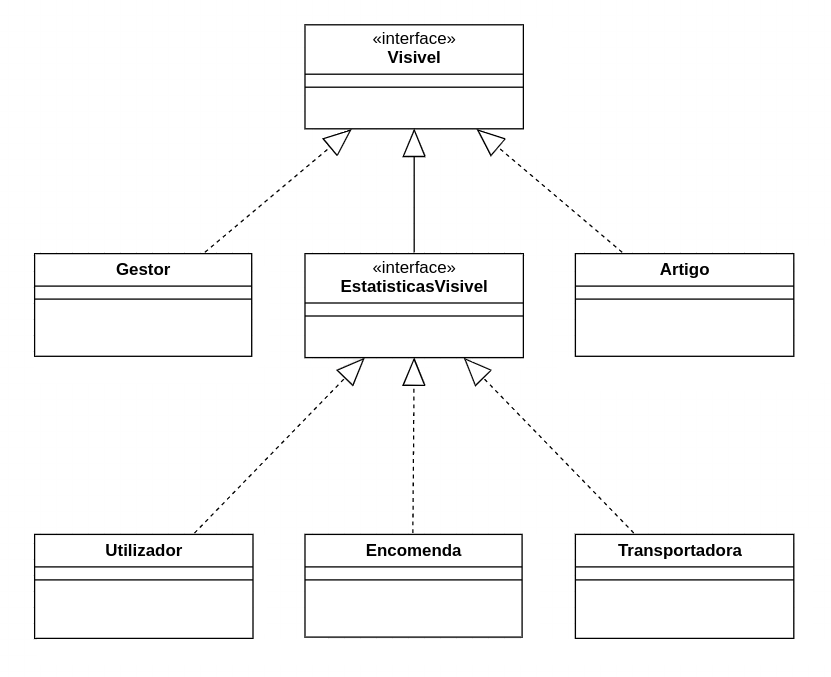
\includegraphics[width=0.7\textwidth]{imagens/9.png}
        \caption*{Figura 11. Hierarquia de Interfaces}
    \end{figure}

    Após muito ponderarmos, chegámos à noção de uma interface \textit{Visivel}, ou seja, todos os objetos que implementem esta interface são reconhecidos pelo \textit{Escritor}, e portanto podem ser apresentados sem que este saiba que classes estão implícitas.

    Contudo existem classes que, para além de serem "visiveis", têm de apresentar estatísticas, e portanto é necessário criar uma outra interface que estenda a noção de \textit{Visivel} e permita a apresentação dessas mesmas estatísticas, daí a criação da interface \textit{EstatisticasVisivel.}